\section{Tangent Spaces} %

% --- TEACHER'S INTRO ---
\noindent
\textbf{Teacher's Note:} Before we dive into the heavy formulas, let's build some intuition. Imagine you are walking on a smooth, curved mountain (a manifold). At any exact point you stand, if you look straight ahead, left, or right, you are looking along a flat plane that perfectly grazes the mountain at your feet. That flat plane is the \qt{tangent space}. The direction sticking straight up into the sky, perpendicular to your flat plane, is the \qt{normal} vector. 
% -----------------------

\subsection{Formal Definition}

% We define a new counter to save the current document's section number dynamically.
% (Note: \newcounter is best placed in the preamble, but works here if only called once!)
\newcounter{savedSection}
\setcounter{savedSection}{\value{section}}

% Setting counters to match the original notes exactly
\setcounter{section}{12}
\setcounter{theorem}{12} % The next definition will be 12.13

\begin{definition}[Tangent and Normal Vectors] %
Let $M \subset \mathbb{R}^n$ be a $d$-dimensional $C^1$ submanifold. %
For a given point $p \in M$, we say that a vector $\tau \in \mathbb{R}^n$ is \qt{tangent} to $M$ at $p$ if there exists a sequence $p_k \in M$ with $p_k \to p$, $p_k \neq p$, and a sequence of positive numbers $r_k$ converging to zero such that %
\[
\lim_{k \to \infty} \frac{p_k - p}{r_k} = \tau. %
\]
The set of all tangent vectors to $M$ at $p$ is called the \qt{tangent space} of $M$ at $p$ and is denoted by %
\[
T_pM := \{ \tau \in \mathbb{R}^n \mid \tau \text{ is \qt{tangent} to } M \text{ at } p \}. %
\]
Furthermore, we say that a vector $\nu \in \mathbb{R}^n$ is \qt{normal} (i.e., perpendicular) to $M$ at $p$ if %
\[
\tau \cdot \nu = 0 \quad \text{for all } \tau \in T_pM. %
\]
The set of all normal vectors at $p$ is called the \qt{normal space} of $M$ at $p$. %
\end{definition}

% Dynamically restoring the section counter back to whatever it was originally
\setcounter{section}{\value{savedSection}}

This is the formal definition of \qt{tangent} and \qt{normal} spaces at a point $p$ of some given $C^1$ submanifold. % 
However, as you saw in the lectures, there is a much better way to find the \qt{tangent space} using partial derivatives. %

\subsection{Practical Computation for Parametrized Surfaces}

For parametrized surfaces (essentially 2-dimensional submanifolds in $\mathbb{R}^n$), the best way to compute the \qt{tangent space} and \qt{normal space} at any point is using the following proposition. %

% Temporarily jump to section 12, def 15 to get Proposition 12.16
\setcounter{savedSection}{\value{section}}
\setcounter{section}{12}
\setcounter{theorem}{15}

\begin{proposition}[Tangent and Normal Vectors for Parametrized Surfaces] %
Let $V \subset \mathbb{R}^2$ be open and let $\phi : V \to \mathbb{R}^3$ be a parametrized surface. %
Then, for every $x \in V$ and $p = \phi(x) \in M$, the following hold: %
\begin{enumerate}
    \item The \qt{tangent space} to $M$ at $p$ is given by the span of the partial derivatives:
    \[
    T_pM = D\phi_x(\mathbb{R}^2) = \text{span}\{\partial_1\phi(x), \partial_2\phi(x)\}. %
    \]
    \item The vectors $\partial_1\phi(x)$ and $\partial_2\phi(x)$ are linearly independent and form a basis of $T_pM$. %
    \item A \qt{normal vector} to $M$ at $p = \phi(x)$ is given by the cross product $\partial_1\phi(x) \times \partial_2\phi(x)$, and a \qt{normal vector} with modulus one (unit normal) is given by %
    \[
    \nu(x) := \frac{\partial_1\phi(x) \times \partial_2\phi(x)}{|\partial_1\phi(x) \times \partial_2\phi(x)|}. %
    \]
    \item Moreover, the \qt{normal space} is the span of this vector:
    \[
    N_pM = \text{span}\{\nu(x)\}. %
    \]
\end{enumerate}
\end{proposition}

% Dynamically resetting section counter back to original
\setcounter{section}{\value{savedSection}}

% --- TEACHER'S VISUALIZATION ---
\begin{center}
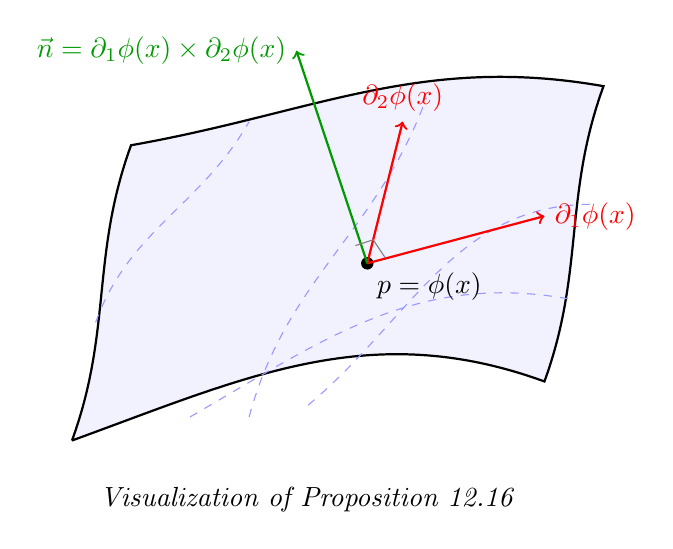
\begin{tikzpicture}[scale=1.5]
    % Draw a wavy surface
    \draw[thick, fill=blue!5] (0,0) to[out=20,in=160] (4,0.5) to[out=70,in=250] (4.5,3) to[out=170,in=10] (0.5,2.5) to[out=250,in=70] (0,0);
    
    % Draw grid lines on the surface
    \draw[blue!40, dashed] (1,0.2) to[out=30,in=170] (4.2, 1.2);
    \draw[blue!40, dashed] (2,0.3) to[out=40,in=180] (4.4, 2);
    \draw[blue!40, dashed] (0.2,1) to[out=70,in=240] (1.5, 2.7);
    \draw[blue!40, dashed] (1.5,0.2) to[out=75,in=250] (3, 2.9);

    % Point p
    \coordinate (P) at (2.5, 1.5);
    \fill[black] (P) circle (1.5pt) node[anchor=north west] {$p = \phi(x)$};

    % Tangent vectors
    \draw[->, thick, red] (P) -- ++(1.5, 0.4) node[right] {$\partial_1\phi(x)$};
    \draw[->, thick, red] (P) -- ++(0.3, 1.2) node[above] {$\partial_2\phi(x)$};
    
    % Normal vector
    \draw[->, thick, green!60!black] (P) -- ++(-0.6, 1.8) node[left] {$\vec{n} = \partial_1\phi(x) \times \partial_2\phi(x)$};
    
    % Right angle marker (approximate for 3D perspective)
    \draw[gray, thin] (2.4, 1.65) -- (2.55, 1.7) -- (2.65, 1.55);
    
    \node at (2,-0.5) {\textit{Visualization of Proposition 12.16}};
\end{tikzpicture}
\end{center}
% -----------------------

\subsection{Examples}

Let's apply this to a foundational example from the notes.

\begin{example}[Spherical Coordinates] %
Consider the parameterization of a unit sphere with a thin slice deleted (the boundary of the unit ball): %
\[
\phi : (0, \pi) \times (-\pi, \pi) \to \mathbb{R}^3, \quad (\theta, \varphi) \mapsto 
\begin{pmatrix}
\sin\theta \cos\varphi \\
\sin\theta \sin\varphi \\
\cos\theta
\end{pmatrix}. %
\]
Let $p = \phi(x) \in M$ for some $x = (\theta, \varphi) \in (0, \pi) \times (-\pi, \pi)$. %
The \qt{tangent space} is $T_pM = D\phi_x(\mathbb{R}^2)$. %
We compute the partial derivatives spanning $T_pM$: %
\begin{align*}
\partial_1\phi(x) &= \frac{\partial}{\partial\theta} 
\begin{pmatrix}
\sin\theta \cos\varphi \\
\sin\theta \sin\varphi \\
\cos\theta
\end{pmatrix}
= 
\begin{pmatrix}
\cos\theta \cos\varphi \\
\cos\theta \sin\varphi \\
-\sin\theta
\end{pmatrix}, %
\\[1em]
\partial_2\phi(x) &= \frac{\partial}{\partial\varphi} 
\begin{pmatrix}
\sin\theta \cos\varphi \\
\sin\theta \sin\varphi \\
\cos\theta
\end{pmatrix}
= 
\begin{pmatrix}
-\sin\theta \sin\varphi \\
\sin\theta \cos\varphi \\
0
\end{pmatrix}. %
\end{align*}

A \qt{normal vector} is then given by the cross product $\vec{n} = \partial_1\phi(x) \times \partial_2\phi(x)$: %
\begin{align*}
\vec{n} &= 
\begin{pmatrix}
\cos\theta \cos\varphi \\
\cos\theta \sin\varphi \\
-\sin\theta
\end{pmatrix} \times 
\begin{pmatrix}
-\sin\theta \sin\varphi \\
\sin\theta \cos\varphi \\
0
\end{pmatrix} %
\\
&= 
\begin{pmatrix}
(\cos\theta\sin\varphi)(0) - (-\sin\theta)(\sin\theta\cos\varphi) \\
(-\sin\theta)(-\sin\theta\sin\varphi) - (\cos\theta\cos\varphi)(0) \\
(\cos\theta\cos\varphi)(\sin\theta\cos\varphi) - (\cos\theta\sin\varphi)(-\sin\theta\sin\varphi)
\end{pmatrix}
\\
&= 
\begin{pmatrix}
\sin^2\theta \cos\varphi \\
\sin^2\theta \sin\varphi \\
\cos\theta\sin\theta\cos^2\varphi + \cos\theta\sin\theta\sin^2\varphi
\end{pmatrix}. %
\end{align*}

\textbf{Teacher's Note:} Notice how in the z-component, we can factor out $\cos\theta\sin\theta$, leaving $(\cos^2\varphi + \sin^2\varphi)$, which simplifies to $1$. 

Thus, the \qt{normal vector} simplifies beautifully to:
\[
\vec{n} = 
\begin{pmatrix}
\sin^2\theta \cos\varphi \\
\sin^2\theta \sin\varphi \\
\sin\theta \cos\theta
\end{pmatrix}
= \sin\theta 
\begin{pmatrix}
\sin\theta \cos\varphi \\
\sin\theta \sin\varphi \\
\cos\theta
\end{pmatrix}. %
\]
The magnitude of this vector is $|\vec{n}| = \sin\theta$. % 
Therefore, the unit \qt{normal vector} $\nu(x)$ is simply the position vector itself:
\[
\nu(x) := \frac{\vec{n}}{|\vec{n}|} = 
\begin{pmatrix}
\sin\theta \cos\varphi \\
\sin\theta \sin\varphi \\
\cos\theta
\end{pmatrix}
= \phi(\theta, \varphi) = \phi(x). %
\]
Geometrically, this makes perfect sense! For a sphere centered at the origin, the direction pointing strictly outward from the surface is exactly the same direction as the position vector of the point itself.
\end{example}

% --- TEACHER'S EXTRA EXAMPLES ---
\begin{example}[Teacher's Extra Practice: The Paraboloid]
To make sure you really have the hang of this, let's look at another classic surface: the paraboloid given by $z = x^2 + y^2$. 
We can parameterize this surface by simply using $x$ and $y$ as our parameters. Let $\phi(x,y) = (x, y, x^2 + y^2)^T$.

1. \textbf{Find the Tangent Vectors:}
\[
\partial_x\phi(x,y) = \begin{pmatrix} 1 \\ 0 \\ 2x \end{pmatrix}, \quad \partial_y\phi(x,y) = \begin{pmatrix} 0 \\ 1 \\ 2y \end{pmatrix}
\]
These two vectors form the basis of the \qt{tangent space} $T_pM$.

2. \textbf{Find the Normal Vector:}
\[
\vec{n} = \partial_x\phi \times \partial_y\phi = \begin{pmatrix} 1 \\ 0 \\ 2x \end{pmatrix} \times \begin{pmatrix} 0 \\ 1 \\ 2y \end{pmatrix} = \begin{pmatrix} -2x \\ -2y \\ 1 \end{pmatrix}
\]
This vector spans the \qt{normal space} $N_pM$ at any point on the paraboloid!
\end{example}

\begin{example}[Teacher's Extra Practice: The Cylinder]
Let's consider a cylinder of radius $R$, described by $x^2 + y^2 = R^2$. 
A natural parameterization uses the angle $\theta$ and the height $z$:
\[
\phi(\theta, z) = \begin{pmatrix} R\cos\theta \\ R\sin\theta \\ z \end{pmatrix}.
\]

1. \textbf{Find the Tangent Vectors:}
Taking partial derivatives with respect to our parameters $\theta$ and $z$:
\[
\partial_\theta\phi(\theta,z) = \begin{pmatrix} -R\sin\theta \\ R\cos\theta \\ 0 \end{pmatrix}, \quad \partial_z\phi(\theta,z) = \begin{pmatrix} 0 \\ 0 \\ 1 \end{pmatrix}
\]
Notice that $\partial_z\phi$ points straight up (parallel to the z-axis), and $\partial_\theta\phi$ is \qt{tangent} to the circular cross-section.

2. \textbf{Find the Normal Vector:}
Taking the cross product:
\[
\vec{n} = \partial_\theta\phi \times \partial_z\phi = 
\begin{pmatrix} -R\sin\theta \\ R\cos\theta \\ 0 \end{pmatrix} \times \begin{pmatrix} 0 \\ 0 \\ 1 \end{pmatrix} = 
\begin{pmatrix} R\cos\theta \\ R\sin\theta \\ 0 \end{pmatrix}
\]
The \qt{normal vector} points directly away from the z-axis in the xy-plane, completely ignoring the z-height. Its magnitude is $|\vec{n}| = \sqrt{R^2\cos^2\theta + R^2\sin^2\theta} = R$. Thus, the unit normal is simply $(\cos\theta, \sin\theta, 0)^T$.
\end{example}
% -----------------------


% --- TEACHER'S SECOND VISUALIZATION (UPDATED) ---
\begin{center}
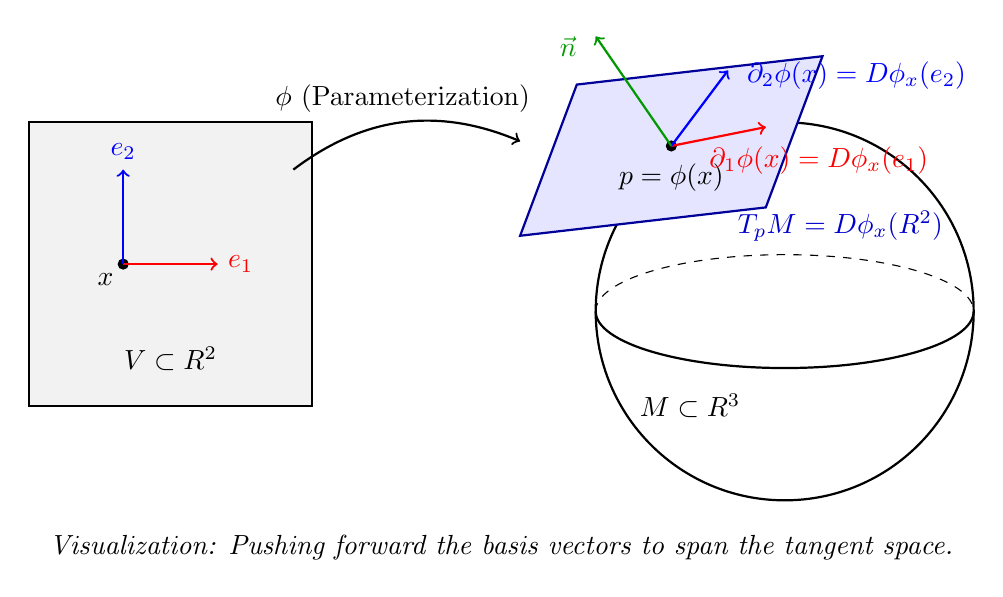
\begin{tikzpicture}[scale=1.2]
    % Left side: The Parameter Domain V in R^2
    \draw[thick, fill=gray!10] (-5, -1) rectangle (-2, 2.0);
    \node at (-3.5, -0.5) {$V \subset \mathbb{R}^2$};
    
    % Point x in V
    \coordinate (X) at (-4, 0.5);
    \filldraw (X) circle (1.5pt) node[below left] {$x$};
    
    % Basis Vectors in R^2
    \draw[->, thick, red] (X) -- ++(1, 0) node[right] {$e_1$};
    \draw[->, thick, blue] (X) -- ++(0, 1) node[above] {$e_2$};
    
    % The mapping phi
    \draw[->, thick, bend left=30] (-2.2, 1.5) to node[above] {$\phi$ (Parameterization)} (0.2, 1.8);
    
    % Right side: The Sphere (Manifold M in R^3)
    \draw[thick] (3,0) circle (2);
    % Equator to give 3D feel
    \draw[dashed] (1,0) arc (180:0:2 and 0.6);
    \draw[thick] (5,0) arc (0:-180:2 and 0.6);
    
    % Label M moved safely inside the lower-left of the sphere
    \node at (2.0, -1.0) {$M \subset \mathbb{R}^3$};
    
    % Point p on the sphere (Front-top-left)
    \coordinate (P) at (1.8, 1.75);
    
    % Tangent plane at p 
    \draw[fill=blue!10, draw=blue!60!black, thick] 
        (0.2, 0.8) -- (2.8, 1.1) -- (3.4, 2.7) -- (0.8, 2.4) -- cycle;
        
    % Tangent plane label moved to the clear bottom-right corner of the plane
    \node[blue!80!black, right] at (2.4, 0.9) {$T_p M = D\phi_x(\mathbb{R}^2)$};
    
    % Draw point p ON the solid plane
    \filldraw (P) circle (1.5pt) node[below, yshift=-0.1cm] {$p = \phi(x)$};
    
    % Pushforward of the basis vectors (The partial derivatives!)
    \draw[->, thick, red] (P) -- ++(1.0, 0.2);
    % Explicitly placed red text inside the sphere
    \node[red, right] at (2.1, 1.6) {$\partial_1\phi(x) = D\phi_x(e_1)$};
    
    \draw[->, thick, blue] (P) -- ++(0.6, 0.8);
    % Explicitly placed blue text out of the way to the right
    \node[blue, right] at (2.5, 2.5) {$\partial_2\phi(x) = D\phi_x(e_2)$};
    
    % Normal vector 
    \draw[->, thick, green!60!black] (P) -- ++(-0.8, 1.16);
    % Explicitly placed green text safely to the left
    \node[green!60!black, left] at (0.9, 2.8) {$\vec{n}$};

    \node at (0, -2.5) {\textit{Visualization: Pushing forward the basis vectors to span the tangent space.}};
\end{tikzpicture}
\end{center}